\chapter{IMRs T1 de la prostate de l'INSERM de Lille.}

Tous les résultats, codes et bases de données d'images IRM peuvent être trouvés sur le git suivant:

\medskip

https://github.com/chuzelph-ENSTA-Bretagne/ThromboseIRM.git

\medskip

\section{Types de courbe rencontrées dans le cadre du cancer de la prostate}


Le document \cite{doi2007computer} présente les différentes courbes caractéristiques de la prostate. Les courbes d'intensité présentent toutes un hyper signal en IRM T1. Néanmoins, les courbes issus de tissus cancéreux présentent un pic d'absorption beaucoup plus marqué avec un temps d'assimilation très caractéristique alors que les tissus sain présentent une courbe d'absorption beaucoup plus lissée. La figure suivante issue de \cite{doi2007computer} donne une illustration de ces courbes caractéristiques.

\medskip

\begin{figure}[H]
\centering
    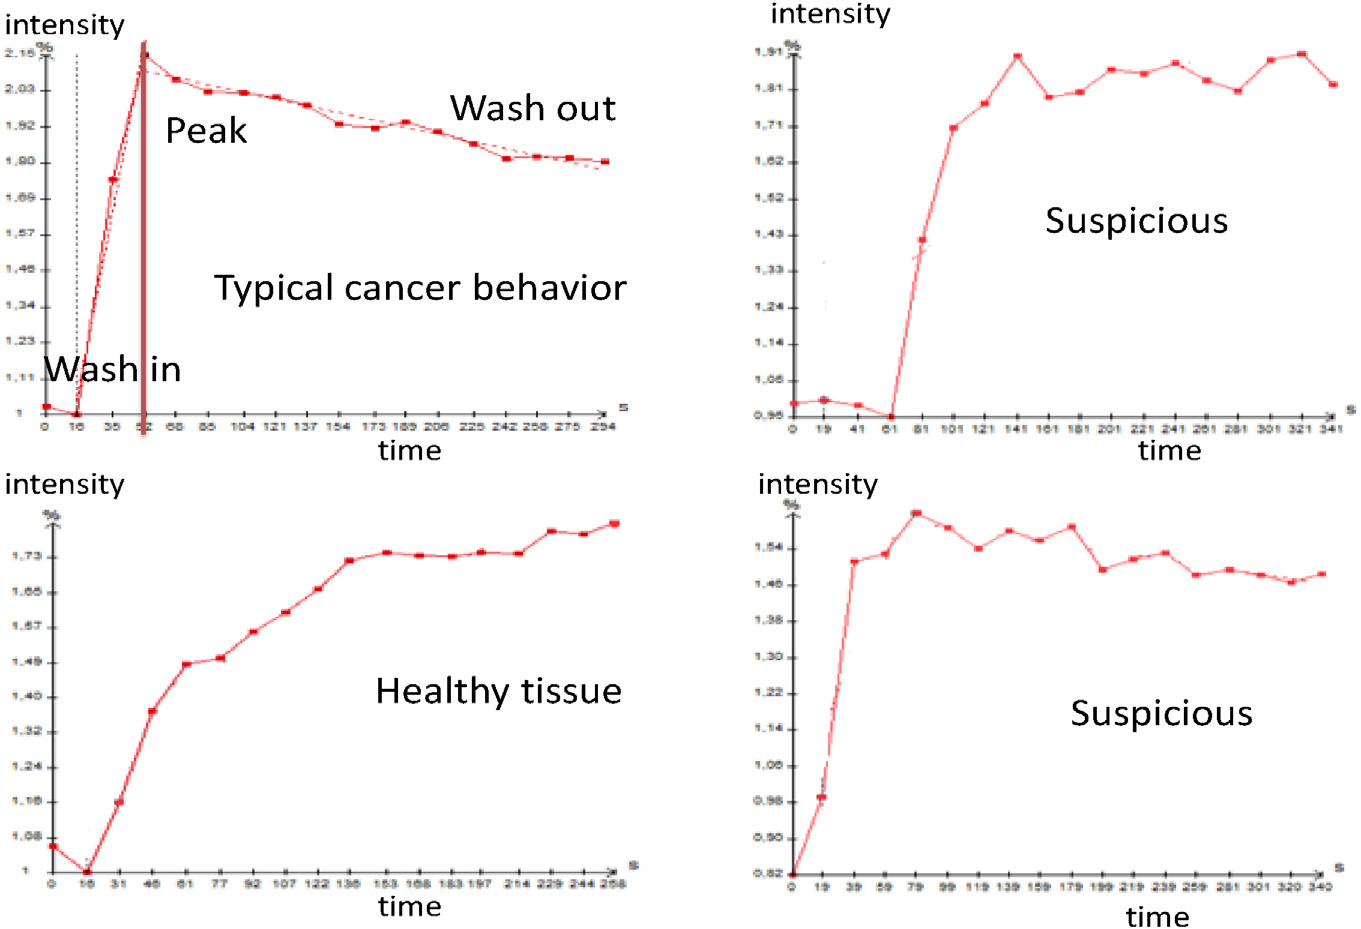
\includegraphics[scale=0.35,angle=0]{Images/CourbeProstate.png}
    \caption{Courbes caractéristiques des tissus sain et cancéreux de la prostate.}
    \label{fig:CourbeProstate}
\end{figure}

\medskip

Néanmoins, certaines courbes sont difficilement à classifier. L'intérêt de notre algorithme va donc être de pouvoir distinguer aisément les tissus sains et les tissus cancéreux et d'estimer avec une autre classe supplémentaire les cas d'incertitude.


\section{Résultats de l'algorithme}

Pour appliquer nos algorithmes, il y a un petit pré-traitement à faire. Pour discriminer les différentes courbes, il faut surtout voir le phénomène de diffusion au sein du tissu et normaliser les courbes afin de faire ressortir le comportement du tissu.
\medskip

Tous les courbes sont donc remise à l'échelle en appliquant la formule suivante:

\begin{equation}
\centering
x(t) \gets \frac{x(t)-x_{min}}{x_{max}-x_{min}}
\end{equation} 

\medskip

Tous les signaux temporels sont donc placés dans une matrice, comme expliqué dans la figure \ref{fig:toolchain}. 
Au final, en appliquant nos algorithmes à une IRM de perfusion de la prostate, nous arrivons au résultat suivant :

\begin{figure}[H]
\centering
    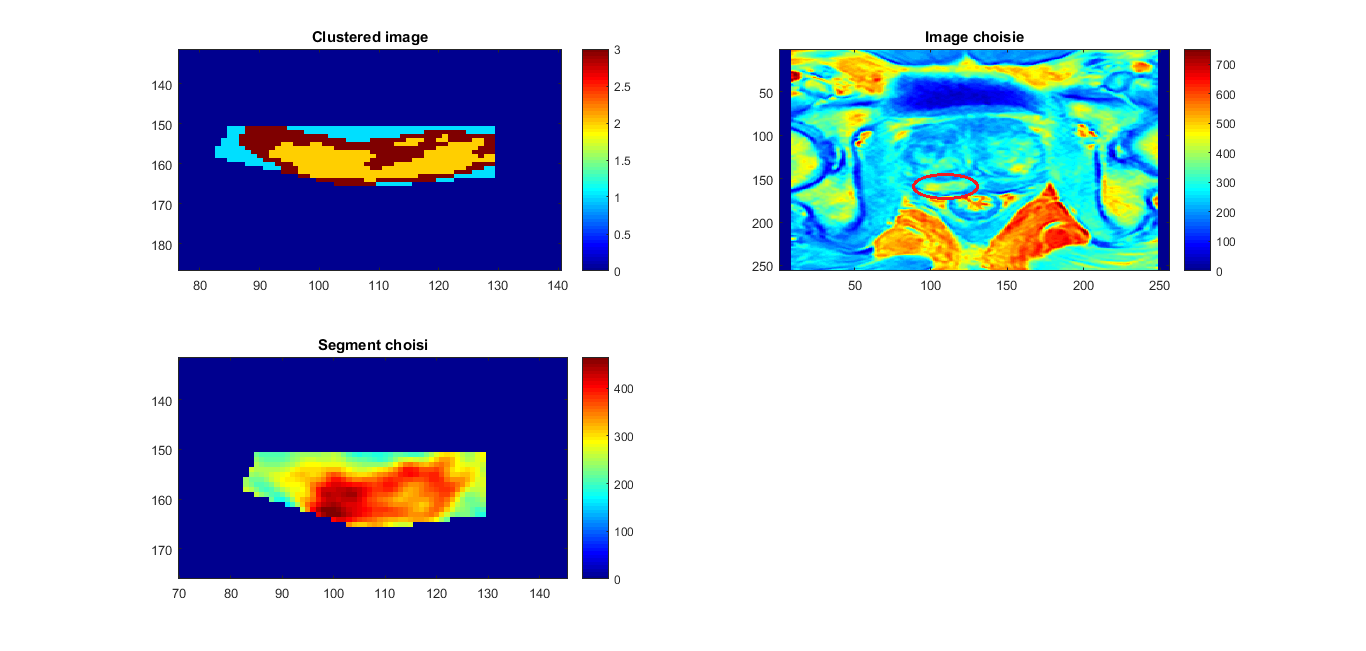
\includegraphics[scale=0.4,angle=0]{Images/3classProstate2.png}
    \caption{Coupes sélectionnées. En haut à gauche le résultat de l'algorithme de classification. En haut à droit, image de la coupe sélectionnée avec la ROI représentée par l'ellipse rouge. En bas à gauche, ROI en fausses couleurs.}
    \label{fig:3classProstate2}
\end{figure} 

La figure suivante montre comment les courbes sont réparties selon les différents clusters.

\begin{figure}[H]
\centering
    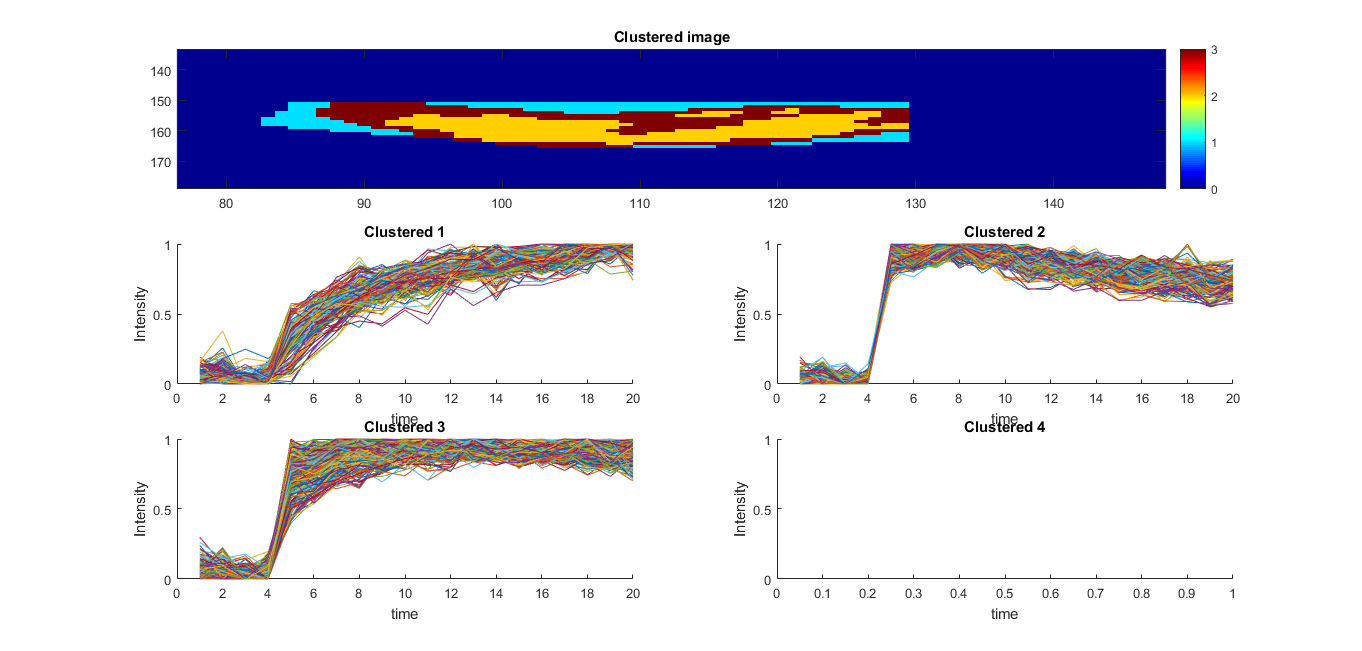
\includegraphics[scale=0.4,angle=0]{Images/3classProstate.png}
    \caption{Résultat de l'algorithme sur l'IRM avec les courbes associées aux clusters.}
    \label{fig:3classProstate}
\end{figure}

Nous avons ici lancé une simulation avec 3 classes. Nous pouvons interpréter ces résultats de la façon suivante:

\begin{itemize}
\item Le cluster 1 rassemble les courbes qui sont saines en accord avec les informations issus de la figure \ref{fig:CourbeProstate},
\item Le cluster 2 lui rassemble les courbes des tissus tumoraux qui présentent un temps d'absorption très court et un pic très marqué,
\item Le cluster 3 lui représentent des courbes qui sont suspectes. Ici, l'algorithme comme l'humain va avoir du mal à trancher sur l'appartenance de ces tissus au sain ou tumoral.
\end{itemize}

Le résultat obtenu est très satisfaisant et on arrive à un résultat semblable à ceux obtenus dans \cite{doi2007computer} bien que la chaine de traitement ne soit pas la même. 

Néanmoins, il y a quelques remarques à faire:

\begin{itemize}
\item Il faut parfois choisir une bonne représentation des données de départ afin que l'algorithme converge vers une solution satisfaisante.
\item Il est nécessaire de choisir une ROI qui est composée d'une zone de taille pas trop importante. En effet, l'algorithme ne converge pas si il y a trop de points sélectionnés.
\end{itemize}


\chapter{IMRs T2 du crane CHRU Brest Cavale Blanche.}

Le CHRU de Brest nous a permis de constituer un base de données de 13 patients présentant des lésions cérébrales caractéristiques sur lesquels nous avons pu tester notre chaine de traitement. Les deux exemples qui vont être présentés ici sont particulièrement pertinents sur les capacités et limites de la méthode pour cette partie du corps. Les IRM que nous utilisons ici sont des IRM T2 ce qui implique que nous aurons la présence d'un hypo-signal pendant la diffusion du produit de contraste.

% Figure avec IRM en niveau de gris de la tumeur
\begin{figure}[H]
\centering
    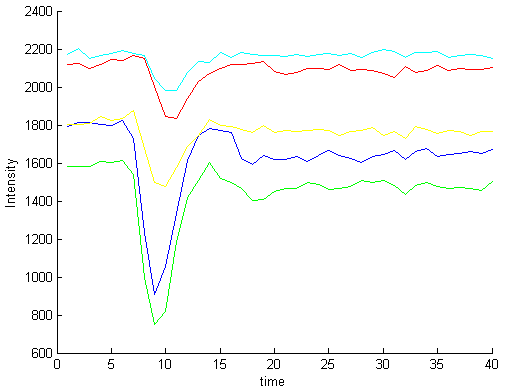
\includegraphics[scale=0.8,angle=0]{Images/CourbeExample.png}
    \caption{Exemples de courbes obtenues par les IRM du CHRU.}
    \label{fig:CourbeExample}
\end{figure}

Nous pouvons créer deux cartes paramétriques à partir des IRM de perfusion qui peuvent aider pour faire un diagnostic. Le premier paramètre est le CBV ou \textit{cerebral brain volume}. Ce paramètre permet de traduire l'importance d'absorption de produit de contraste par le tissu considéré. Le document \cite{muir2014quantitative} définit le CBV par la méthodologie suivante. Le temps de relaxation transversal $\Delta R2^*$ est donné par la formule:

\begin{equation}
\Delta R2^*(t) = \frac{-ln(S(t)/S_0}{TE}
\end{equation}

où $TE$ est le temps de pulsation d'écho de l'IRM. Il est récupérable sur les méta-données de l'IRM. Le CBV est donc défini comme l'intégrale de $R2^*(t)$

\begin{equation}
CBV = \int^{t_f}_{t_0} R2^*(t) dt
\end{equation}

Le second paramètre est le CBF ou \textit{cerebral brain flow}. Il n'est pas pertinent pour l'étude que nous avons menée mais il a été implémenté sur Matlab.

\medskip



\section{Patient 1: Cancer identifiable par l'IRM de perfusion.}

L'IRM qui est ici présentée provient d'un patient qui a un cancer bénin situé à la frontière du cerveau et de la boite crânienne. La tumeur est visible sur la figure suivante à sur la partie gauche de l'image. A sa droite, on peut voir la présence d'un assez gros œdème résultant de la présence de la tumeur. Le reste du cerveau est sain et il y a au centre de l'image le ventricule cérébrale qui produit le liquide céphalo-rachidien. Ce dernier apparait ici avec un hyper-signal caractéristique.

% Figure avec IRM en niveau de gris de la tumeur
\begin{figure}[H]
\centering
    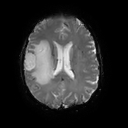
\includegraphics[scale=2,angle=0]{Images/Patient4IRM.png}
    \caption{IRM du patient présent une tumeur bénigne et un œdème.}
    \label{fig:patient4IRM}
\end{figure}

Nous avons donc appliqué notre algorithme en sélectionnant une ROI qui ne contient pas le ventricule cérébral afin qu'il ne vienne pas parasité le résultat de l'algorithme. Nous avons également demandé qu'il ressorte quatre classes. La figure qui suit montre dans l'ordre, l'IRM du patient en fausse couleur, la carte paramétrique du CBV et le résultat de notre algorithme.

% Figure du patient 4 avec les résultats du programme.
\begin{figure}[H]
\centering
    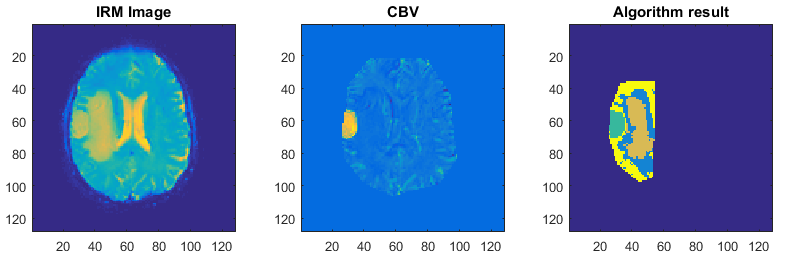
\includegraphics[scale=0.8,angle=0]{Images/Patient4Result.png}
    \caption{Résultat de l'algorithme.}
    \label{fig:patient4IRMResult}
\end{figure}

La carte de CBV est ici particulièrement adaptée car elle fait ressortir tout tissu qui a tendance à absorber un grand volume de produit de contraste par rapport au reste du cerveau. Sur cette carte, on voit que la tumeur est immédiatement isolée.

On peut remarquer que l'algorithme que nous avons mis en place permet d'isoler parfaitement la tumeur mais également l'œdème et permet d'établir une zone de frontière entre cette œdème et les tissus sains.

\bigskip
\begin{Large}
\textcolor{blue}{Conclusion:}
\end{Large}
\medskip

On peut voir par cette exemple que notre algorithme est particulièrement adapté pour cette pathologie car cette tumeur impacte beaucoup la diffusion du produit de contraste. Néanmoins, on peut regretter que nous ne pouvons détecter que un unique œdème avec notre algorithme.


\section{Patient 2: Cancer non-identifiable par l'IRM de perfusion.}

L'IRM qui suit provient d'un patient qui a un cancer situé dans la région en haut à gauche du cerveau. On peut voir un très gros œdème qui est situé tout autour de la tumeur mais cette dernière n'implique pas de modification notable de la diffusion du produit de contraste ce qui se traduit par un CBV qui n'est pas particulièrement modifié.

% Figure avec IRM en niveau de gris de la tumeur
\begin{figure}[H]
\centering
    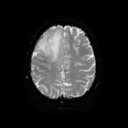
\includegraphics[scale=2,angle=0]{Images/Patient2IRM.png}
    \caption{IRM du patient présent une tumeur et un œdème. Ici, seul l'œdème est identifié par notre algorithme.}
    \label{fig:patient4IRM}
\end{figure}

\begin{figure}[H]
\centering
    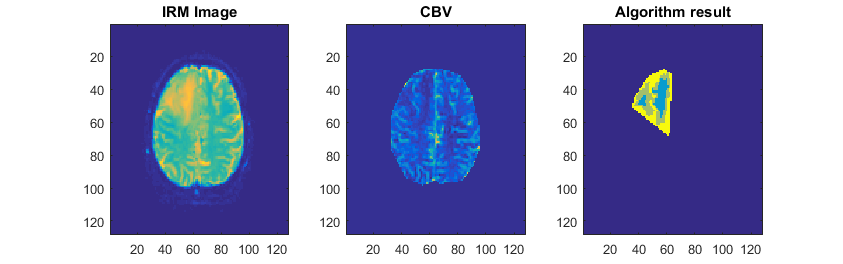
\includegraphics[scale=0.8,angle=0]{Images/Patient2Result.png}
    \caption{Résultat de l'algorithme.}
    \label{fig:patient4IRMResult}
\end{figure}

Nous avons testé notre algorithme en demandant la création de 2 et 3 classes et on retrouve un résultat similaire à celui ci-dessus. On observe que dans le cas où on demande deux classes, on a l'œdème qui est identifié et pour 3 classes, on a une zone frontière qui se créer entre le tissu sain et l'œdème. Néanmoins, la tumeur ne peut être identifier.

\begin{figure}[H]
\centering
\begin{subfigure}{.5\textwidth}
    \centering
    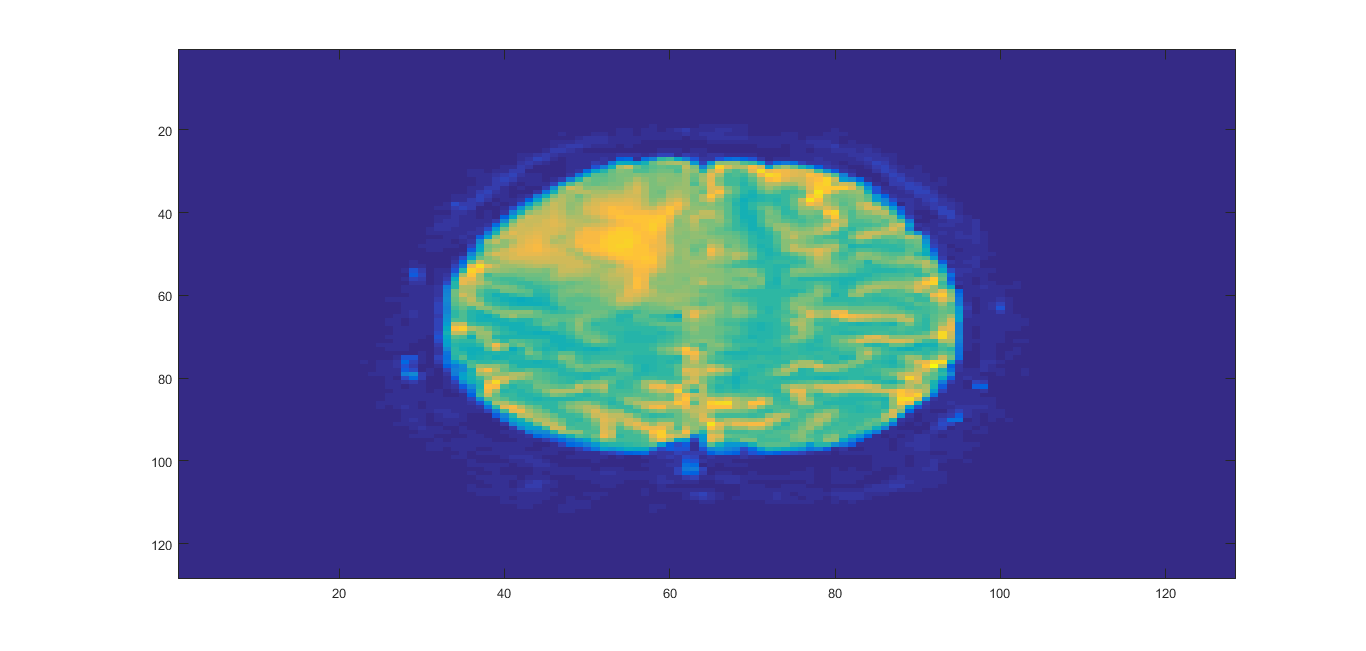
\includegraphics[scale=0.2,angle=0]{Images/TrueclassBrain.png}
    \caption{Image originale.}
    \label{fig:TrueclassBrain} 
\end{subfigure}
\begin{subfigure}{.33\textwidth}
    \centering
    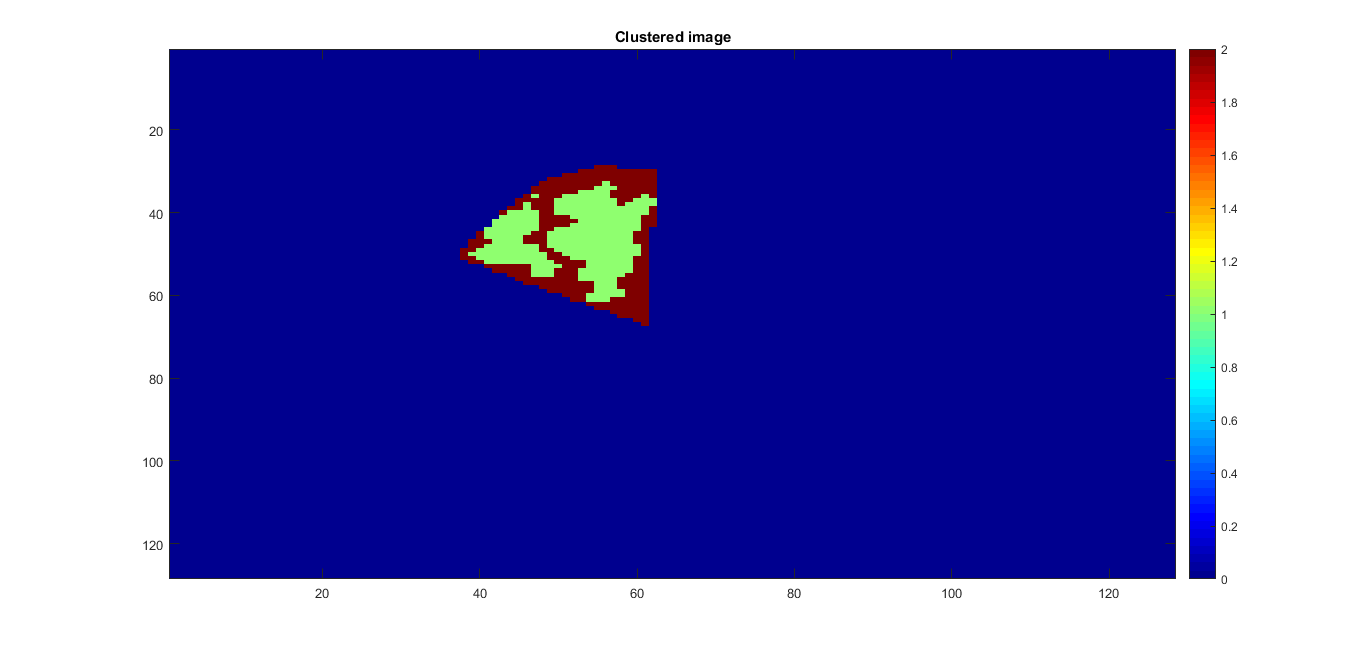
\includegraphics[scale=0.2,angle=0]{Images/2classBrain.png}
    \caption{Résultat de l'algorithme avec 2 classes.}
    \label{fig:2classBrain} 
\end{subfigure}
\begin{subfigure}{.33\textwidth}
    \centering
    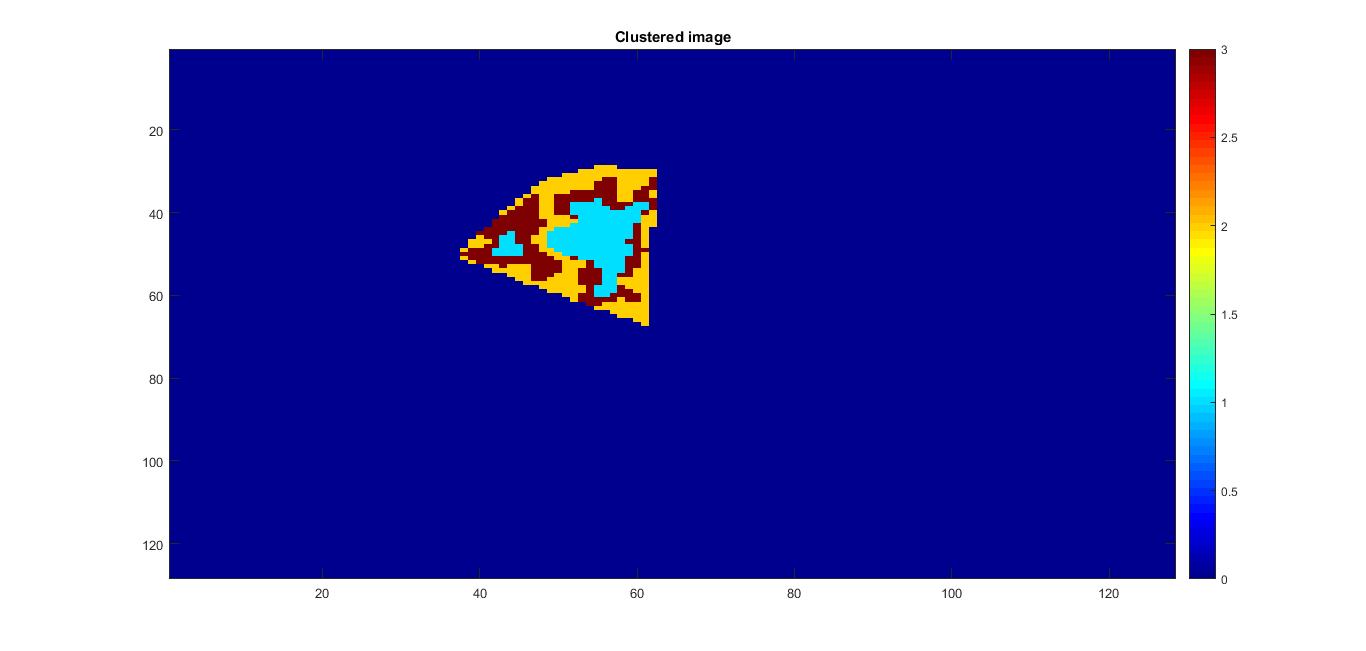
\includegraphics[scale=0.2,angle=0]{Images/3classBrain.png}
    \caption{Résultat de l'algorithme avec 3 classes.}
    \label{fig:3classBrain} 
\end{subfigure}
    \caption{Résultats de notre algorithme sur le patient 2 avec 2 et 3 classes.}
    \label{fig:2and3classBrain} 
\end{figure}

\bigskip
\begin{Large}
\textcolor{blue}{Conclusion:}
\end{Large}
\medskip


Tant notre algorithme que la carte de CBV sont ici inadapté pour cette pathologie. Bien que on identifie clairement l'œdème, le principal but de notre algorithme est de pouvoir identifier des pathologies plus graves comme les tumeurs. Mais dans certains cas comme celui ci-dessus, il est nécessaire de trouver d'autres sources d'information plus pertinentes pour proposer une segmentation de la zone pathologique.
